\documentclass[11pt]{article}
\usepackage[T1]{fontenc}
\usepackage[utf8]{inputenc}
\usepackage{lmodern}
\usepackage{microtype}
\usepackage{amsmath}
\usepackage[margin=1in]{geometry}
\usepackage{booktabs}
\usepackage{array}
\usepackage{graphicx}
\usepackage{xcolor}
\usepackage[colorlinks=true, linkcolor=blue!50!black, citecolor=blue!50!black, urlcolor=blue!50!black]{hyperref}
\usepackage{parskip}

\newcommand{\code}[1]{\texttt{#1}}

\title{\textbf{Compress the Access, Not the Store}\\[2pt]
\large A measurement of key-lookup versus file-search retrieval cost\\
for AI agents, on a real engineering project}
\author{Vasili Gavrilov\\\small ORCID 0009-0007-9371-5994}
\date{June 2026}

\begin{document}
\maketitle

\begin{abstract}
\noindent
This paper measures, on a real codebase, a claim the field asserts but seldom
tests: how many tokens an AI agent spends to find an answer by searching the files
versus recalling it from a curated key index. Agents pay for context in tokens, and
the bill grows with the store; file search and vector retrieval scan the whole
thing, sometimes badly. On a project of about 100k lines of code we run an agent
loop over the same questions twice, once with \code{grep} and read, once with the
index, and count. The result depends on how the index is used, which is a design
choice: when it returns the answer or a reference a person consumes, retrieval is
about $69\times$ cheaper on the content pulled into context, more reliable (40 of 40
correct across repeats versus 31 of 40, on a substring grading that by construction
favours the curated index), and flat in repository size, while search grows and
occasionally explodes (one query reached 170{,}000 total tokens); run directly on
the command line it costs zero model tokens. Making the model read the recalled
document instead shrinks the gain to about $3\times$, an avoidable misuse. The idea
is old, a user-owned plain-text index, exact and self-verifying (a wrong key returns
the empty set, a checksum), a durable format predating RAG, that compresses the
\emph{access} (the keys), not the store. What is new is the measurement and the
stance it serves: (1)~it is cheaper and more reliable than the lexical file search
measured here, and, by the same reasoning though not by measurement, than similarity
search; (2)~as a byproduct, the fixed per-turn overhead is itself reducible, by
prompt caching, a minimal recall tool, and recall-first routing, which pushes even
the agent path toward the zero-token floor; and (3),~qualitatively, the index
encodes \emph{this user's} prior rather than the population average, an argument we
make but do not measure.
\end{abstract}

\noindent\textbf{Keywords:} large language model agents; retrieval cost; associative
key index; faceted classification; retrieval-augmented generation; code search;
Model Context Protocol; reproducible measurement.

\section{The question}

Consider a photo library. One picture is of \emph{Mary} and \emph{Mother}, at the
\emph{beach}, in \emph{Hawaii}, in \emph{2019}, all at once; no folder holds it
without forcing one parent and losing the rest. What you want to ask is the
combination, every photo of Mary with Mother, and not the videos. Two strategies
answer it. \emph{Search} the content: scan the items and match by text or
similarity, then filter. Or keep a curated \emph{index}: file each item under one
or more keys and recall it by their intersection. The index is an old idea,
traceable to Bush's memex~[1]; its non-hierarchical, combine-the-facets form is
Ranganathan's faceted classification~[2]. Keys are facets, a query is their set
intersection (\code{mary} $\cap$ \code{mother} $\cap$ \code{photo}); the index is
plain text on the user's own machine, and retrieval is a deterministic lookup, not
a similarity search.

The index measured in this paper, AIS, is a plain-text associative index the
author built for exactly this purpose: personal, un-hierarchical material, photos,
notes, references, filed under keys and recalled by their intersection. A language
model given a large codebase faces the same choice, grep and read its way to an
answer, or recall it from such an index, and the cost is simply easier to count
there. The two put context into the model but compress it differently. Embedding search
compresses the content into a learned embedding space and retrieves by similarity;
the key index retrieves by exact address, \emph{compression in keys}. That distinction, and the case for compressing the
\emph{access} rather than the stored content, is argued in the conceptual
foundation~[12]. The present paper is the \emph{measurement}: it takes that concept
as given and asks the narrow, quantitative question, \emph{for the same question,
how many tokens does each spend to find the answer, and how reliable is each?} We
answer it on a real project, and report the regime-dependent outcome,
including the case where the index does \emph{not} win by much.

\section{The two strategies}

\textbf{Content search (lexical or embedding).} The alternative to a key
index is to search the content itself, lexically (grep) or semantically (an
embedding search over chunks, the dense-retrieval~[5] core of RAG~[4], which
compresses content into a learned embedding space and retrieves by similarity). Either way the agent scans the corpus and
pulls candidates into context. We measure the lexical baseline: the agent is given
\code{grep}, \code{read\_file}, and \code{list\_files}, greps for likely terms,
reads candidates, and answers. Its cost is the content it pulls in, which grows
with the repository and spikes when a common term matches widely. Beyond cost, a
large, undifferentiated context also degrades answer accuracy, the ``lost in the
middle'' effect, where a relevant fact buried in a long input is missed~[14]; a
smaller retrieval payload therefore helps on two axes at once.

\textbf{Compression in keys (the index).} The agent is given the index tools
(\code{recall}, \code{keys}). Keys are exact: a recall either hits the curated
vocabulary or returns the empty set, which is an immediate, correctable signal
(the empty set
acts as a checksum, and the key list is the codebook). The recalled value is a
short note, a URL, or a path; when it is the answer or a reference, the human (or
a downstream step) consumes it directly and the model does not expand it.

\begin{figure}[h]
\centering
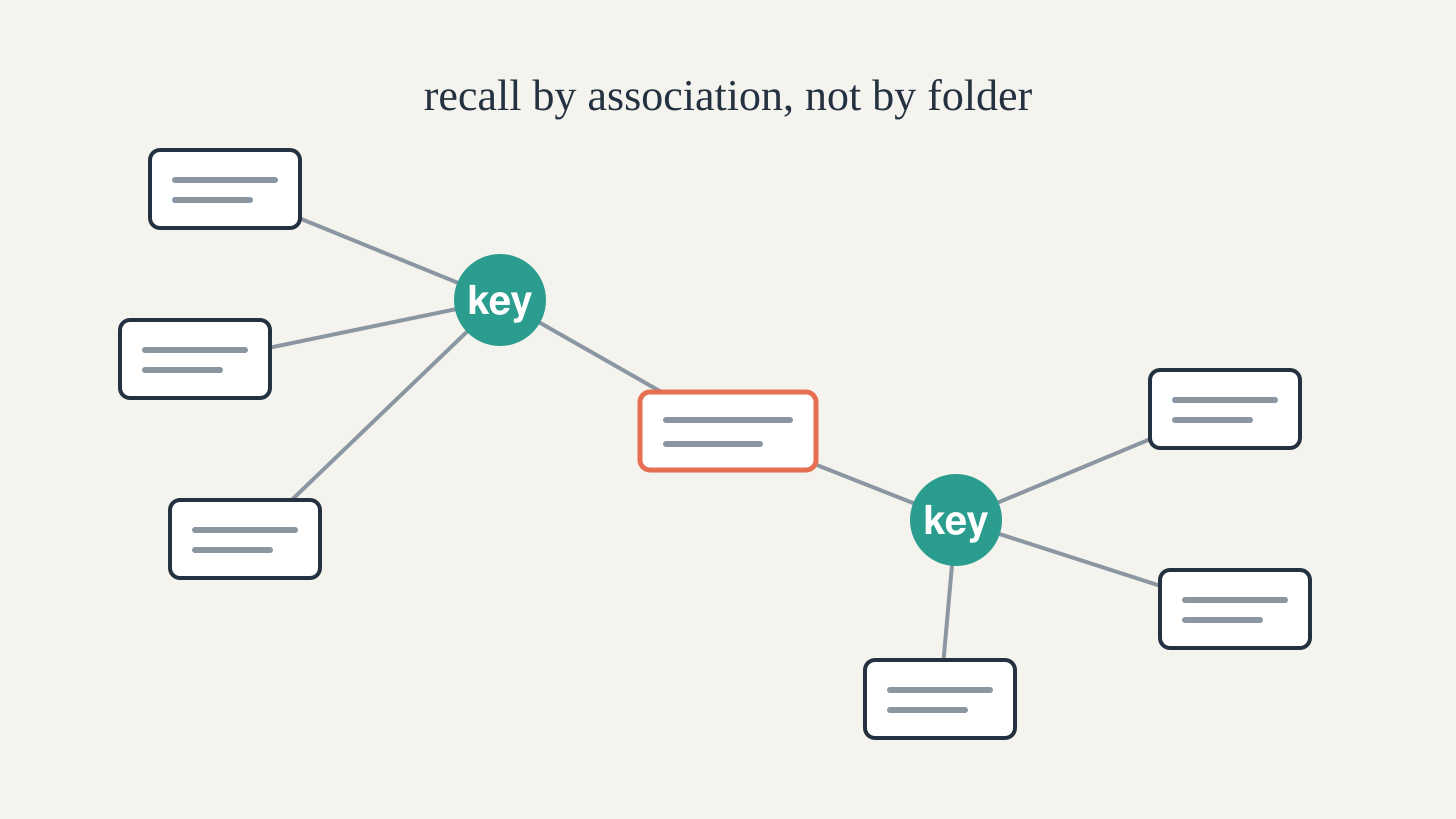
\includegraphics[width=0.66\linewidth]{set_algebra.png}
\caption{Compression in keys. Each item is filed under one or more keys; items
sharing a key are recalled together, and a query is the \emph{intersection} of the
lists of items filed under each key (their posting lists), a deterministic lookup
on the user's machine, not a
similarity search in a learned embedding space.}
\label{fig:keys}
\end{figure}

\section{What we built}

Two pieces of software, both thin wrappers over a single-binary ANSI C
associative-index engine whose store is plain text:

\textbf{The plugin.} A Model Context Protocol (MCP) server~[10]. MCP is the open
standard for offering a language model a set of callable tools; this server exposes
the index's operations, recall by keys, store, list keys, as typed tools to any
MCP-capable chat client (terminal agent or desktop). It is stateless: the
plain-text index remains the source of truth, and the server simply forwards
calls to the engine. It optionally logs each call's payload size and latency,
which is what made the measurement below possible. This is the production
integration: it lets a model reach the user's curated index without the index
ever leaving the machine.

\textbf{The harness.} A \emph{harness}, in software testing, is the small program
that runs an experiment automatically: it poses each question to the model, gives
it a fixed set of tools, executes whatever tool the model asks for, feeds the
result back, and records what was spent. Ours is a minimal \emph{agent loop}, the
pattern in which a model may call a tool, see the result, and call again until it
is ready to answer, driving a commercial model (Claude
Sonnet) through its messages API. For one question it runs:
\begin{enumerate}
\item Send the question, a fixed system instruction, and \emph{one} of two tool
schemas: the index set \,\code{recall(keys)}, \code{keys()}\, or the file-search
set \,\code{grep(pattern)}, \code{read\_file(path)}, \code{list\_files(glob)}.
\item If the model returns a tool call, execute it locally (against the engine, or
the file system), append the result to the conversation, and repeat from step~1.
\item If the model returns text and no tool call, that is the final answer; stop.
\end{enumerate}
Execution is local and identical for both arms except the tool set. In the
representative run the index arm has \emph{no} \code{read\_file}: recall returns
the answer, and a recalled reference is opened by the human, not the model. Each
question is answered in a \emph{fresh} conversation, so runs share no context.
Because the harness drives the same recall tool the plugin exposes, what it
measures is what production use would pay.

\section{Method}

\textbf{What we count.} For each question and arm, summed over all turns of the
loop, we record:
\begin{itemize}
\item \emph{total tokens}: the API's reported input plus output tokens across
every turn. This carries a fixed per-turn overhead, the system instruction, the
tool schemas (re-sent each turn), and the model's own output, of roughly 2{,}500
to 3{,}000 tokens, paid identically by both arms; it therefore \emph{dilutes} the
comparison.
\item \emph{retrieval payload}: the total size, in tokens (bytes\,/\,4), of all
\emph{tool results} returned to the model, the content actually pulled into the
context window to find the answer. This is the quantity the index optimizes, and
unlike total tokens it is not diluted by the fixed overhead. It is the headline
metric.
\item \emph{correctness}: whether the expected answer string appears in the final
response; for set questions, \emph{item-recall}, the fraction of expected items present.
\item tool rounds and wall-clock latency.
\end{itemize}

\textbf{Controls.} Both arms answer the same questions, with the same model, in
fresh conversations. The index directory is excluded from the file-search arm, so
it cannot grep the index itself and must find answers in the genuine project
files. Tool outputs are capped (grep to its first matches, reads to a fixed size)
so no single call can dump the whole repository; this bounds the search arm
\emph{in its favour}, the uncapped gap would be larger. The representative run is 8
questions over 5 repeats; the two preliminary runs were single passes, treated as
illustrative.

\textbf{Project.} The search target is a real product repository. The search arm
greps the working tree the agent actually sees: about $0.35$\,GB across roughly
1{,}300 files and 100k lines of source. (The full checkout is 1.9\,GB on disk, but
1.6\,GB of that is version-control history under \code{.git}, which is excluded and
never searched.) An \emph{uncapped} grep for a single common term over this tree
would return on the order of 17{,}000 to 110{,}000 tokens of raw matches; the
harness caps each tool result to about 1{,}500 tokens, so the search agent pays
this haystack across many capped turns rather than in one dump.

\textbf{What the index stores sets the regime.} We vary it deliberately:
\emph{paths} (the key maps to a document path, and the agent reads the document to
answer) versus \emph{notes and references} (the key maps to a short note or a URL
that \emph{is} the answer, recalled and returned, no reading). Questions are
natural-language and varied (``how do I deploy a release to dev'', ``give me all
the documents about deployment'').

\textbf{Preliminary runs, and the representative one.} We iterated. Two early runs
are reported only to explain the design and should not be read as the result. A
single-fact toy (questions returning one short value) was trivial. A document-set
run in which the index returned a path \emph{and the agent was made to read the
document} understated the effect, because it charged the model for reading, which
is not how the tool is used: a recalled URL or file is opened by the person, not
expanded by the model. The \textbf{representative run}, and the most recent, stores
notes and references that are themselves the answer and has the index arm
\emph{recall only}, no reading. That is real usage, and the rest of this section
reports it.

\section{Results}

\textbf{The representative run (notes/references, no model reading), 8 questions
$\times$ 5 repeats.} The index recalled about \textbf{68 tokens} of content per
question; file search pulled in about \textbf{4{,}744}, a \textbf{69$\times$}
retrieval-payload ratio. The index answered \textbf{40 of 40} (item-recall 1.0) with
a tight spread (mean about 2{,}900 tokens, standard deviation 518); file search
answered \textbf{31 of 40} (item-recall 0.78) with enormous variance (standard
deviation about 36{,}000, larger than its own mean). Table~\ref{tab:notes} and
Figure~\ref{fig:results} give the per-question means. The failures are not confined
to the expensive runs: search missed \code{release\_packaging} on \emph{all five}
repeats (at 6{,}400 to 72{,}000 tokens), yet usually \emph{found} \code{monitoring}
despite spending 17{,}000 to 170{,}000 tokens to do so. Both documents exist in the
project; search fails to surface \code{release\_packaging} within the turn budget,
not for its absence. Cost and correctness fail independently.

\begin{figure}[h]
\centering
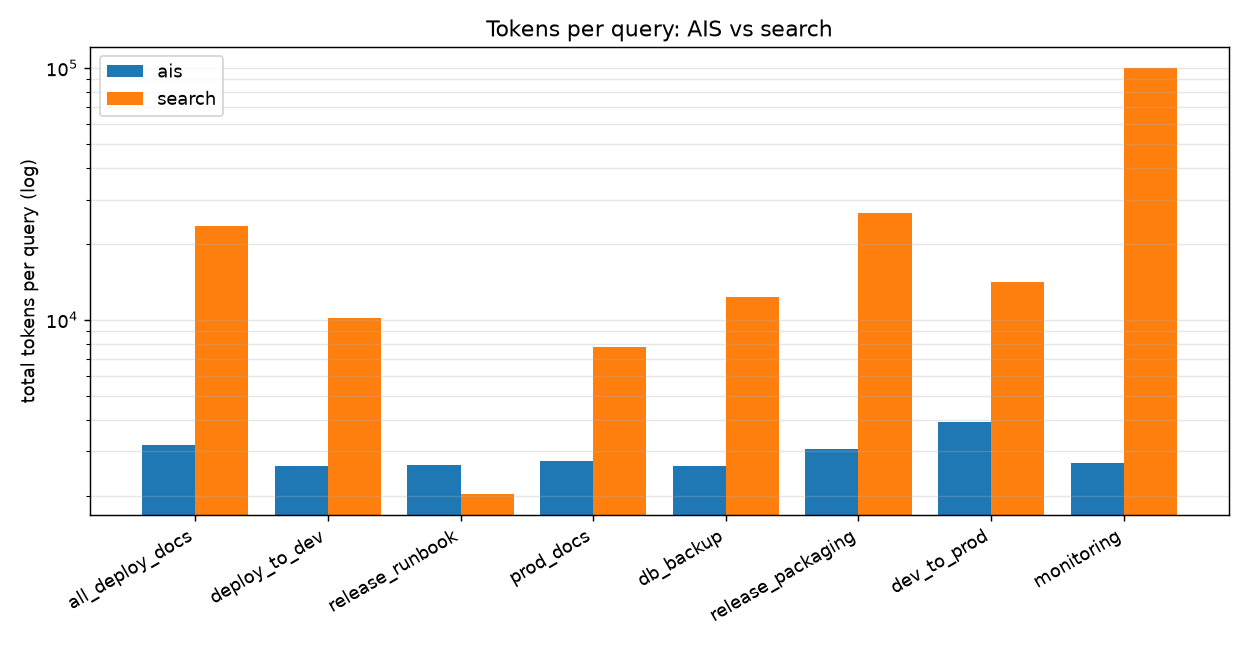
\includegraphics[width=0.82\linewidth]{chart_notes.png}
\caption{Per-question total tokens (log scale), representative run. The index
(left bars) stays low and flat; file search (right bars) is higher and spikes on
common-term greps (\emph{release packaging}, \emph{monitoring}).}
\label{fig:results}
\end{figure}

\begin{table}[h]
\centering
% generated by analyze.py --latex; do not edit by hand
\begin{tabular}{lrrr}
\toprule
\textbf{question} & \textbf{index tok} & \textbf{file-search tok} & \textbf{ratio} \\
\midrule
\code{all\_deploy\_docs} & 3{,}180 & 23{,}611 & 7$\times$ \\
\code{deploy\_to\_dev} & 2{,}635 & 10{,}173 & 4$\times$ \\
\code{release\_runbook} & 2{,}663 & 2{,}039 & 1$\times$ \\
\code{prod\_docs} & 2{,}745 & 7{,}768 & 3$\times$ \\
\code{db\_backup} & 2{,}632 & 12{,}372 & 5$\times$ \\
\code{release\_packaging} & 3{,}059 & 26{,}438 & 9$\times$ (search miss) \\
\code{dev\_to\_prod} & 3{,}931 & 14{,}066 & 4$\times$ \\
\code{monitoring} & 2{,}706 & 99{,}499 & 37$\times$ \\
\midrule
\textbf{mean} & \textbf{2{,}944} & \textbf{24{,}496} & \\
\bottomrule
\end{tabular}

\caption{Per-question total tokens, representative run (note/reference index, no
model reads). A common-term grep over the searched tree both explodes and
misses.}
\label{tab:notes}
\end{table}

\textbf{Why the total-token ratio understates it.} Read on \emph{total} tokens per
turn, the index beats search by a few times (mean 9$\times$, median 4$\times$ in
this run). That total is diluted: both arms pay the same large, fixed model
overhead every turn (system prompt, tool schemas re-sent each turn, the model's
prose answer), about 2{,}500 to 3{,}000 tokens, identical whether the agent
recalls or greps. The retrieval payload (Table~\ref{tab:regimes}) isolates the
quantity the index actually optimizes.

\begin{table}[h]
\centering
\begin{tabular}{lcccc}
\toprule
\textbf{index returns} & \textbf{total ratio} & \textbf{retrieval ratio} & \textbf{index} & \textbf{search} \\
\midrule
\textbf{note / URL, no read (representative)} & \textbf{9$\times$} & \textbf{69$\times$} & \textbf{40/40} & 31/40 \\
direct CLI, no model                          & \multicolumn{1}{c}{0 tokens} & n/a & exact & n/a \\
\bottomrule
\end{tabular}
\caption{Regimes. The representative run is the measured note/reference case;
direct CLI is the zero-token path. The preliminary path-with-read and single-value
runs are described in the text, not tabulated.}
\label{tab:regimes}
\end{table}

\textbf{The path-with-read contrast.} When the index returns a document path and
the agent then reads it, both arms incur the same reading cost; the index saves
only the \emph{finding}, so the retrieval-payload advantage shrinks to about
3$\times$. This is the avoidable case, and naming it is the point: do not make the
model expand a recalled reference.

\textbf{Direct invocation.} For a known, repeated key the user (or a script) runs
the lookup on the command line and the model is never involved: zero model tokens.
The agent comparison cannot show this, because it forces every query through the
model; it is the ceiling of the economy.

\section{Analysis}

\textbf{The regime is a design choice.} Same index, same questions, same project:
the only thing that moved the retrieval advantage from 3$\times$ to 69$\times$ was
\emph{what the key returns and who consumes it}. Store a path and make the model
expand it, and you pay for reading, which search pays too. Store the answer (a
note) or a reference (a URL) and let the person open it, and retrieval is
close to free. Paths answer ``\emph{which} document''; notes answer
``\emph{what} is the answer''.

\textbf{Cost versus repository size.} The index's retrieval cost is roughly
constant in repository size (a key addresses an index entry), while file search
grows with the corpus and spikes pathologically on common terms: across repeats,
individual \code{monitoring} runs reached 170{,}000 \emph{total} tokens (the
question averaged about 99{,}000). These totals are dominated by the transcript
re-sent over 16 to 20 turns; the retrieval payload on those queries is about
15{,}000 to 17{,}000 tokens. As a project grows the gap widens; the index does not
notice the growth.

\textbf{Reliability, not only cost.} The index was exact on every question and
every repeat (40 of 40); file search was wrong on 9 of 40 runs (item-recall 0.78),
and failed one question, \code{release\_packaging}, on all five repeats. This
follows from the mechanics:
exact-key lookup returns either the curated answer or the empty set (a detectable
miss), whereas file search and generation always return \emph{something}
plausible, so an error is never signalled. Exactness buys verifiability, which
approximate retrieval structurally cannot.

\section{Estimated savings}

The measured per-query figures support a rough projection; \emph{rough} is the
operative word. For a curated, repeated lookup the saving is about
$C_{\mathrm{search}} - C_{\mathrm{AIS}}$, where $C_{\mathrm{search}}$ is what the
agent spends finding the answer by file search and $C_{\mathrm{AIS}}$ is what the
index spends. From the representative run, $C_{\mathrm{AIS}}\approx 2{,}900$ tokens
through the model, or $0$ used directly on the command line; $C_{\mathrm{search}}$
had a median near $11{,}500$ and a mean near $24{,}500$ tokens (individual
pathological greps reached $170{,}000$) and grows with repository size. So each
curated query saves on the order of $8{,}500$ tokens through the model, and
nearly all of $C_{\mathrm{search}}$ when the lookup is run directly.

\begin{table}[h]
\centering
\begin{tabular}{lrr}
\toprule
\textbf{lookups/day} & \textbf{via model (saves $\sim$8.5k)} & \textbf{direct CLI (saves $\sim$11.5k)} \\
\midrule
30  & $\sim$0.25M tok/day & $\sim$0.35M tok/day \\
100 & $\sim$0.85M tok/day & $\sim$1.2M tok/day \\
\bottomrule
\end{tabular}
\caption{Projected daily token saving per developer for curated, repeated lookups.
The 30 to 100 range is a conservative, human-scale floor: Sadowski et al.~[3] report
a median near 12 code searches per weekday, and counting docs, configs, and
references adds more. The \emph{agentic} regime this paper targets runs far higher,
one task issues many retrievals and a developer may run several agents, so the
saving grows rather than shrinks. We know of no published per-day agent-lookup rate
yet, so this is a structural estimate, not a measured deployment; quantifying real
lookup volume, human and agent, is a natural next step. Over about 20 working days
the range is roughly 5 to 20 million tokens per developer per month, tens of dollars
per heavy user at commercial rates (mostly input tokens).}
\label{tab:savings}
\end{table}

Three qualifications. The saving applies only to \emph{curated, repeated} lookups,
the value regime; first-time or unknown-key questions fall back to search and save
nothing (the empty result instead tells you what to add). $C_{\mathrm{search}}$ is
noisy, so the claim is ``one to two orders of magnitude per curated
query'', not a point estimate. And the largest lever is not the token ratio but
avoiding the model entirely for recall: a direct lookup costs zero, which the agent
comparison cannot represent.

\section{Threats to validity}

These are small pilots: 8 questions over 5 repeats, on one project, with one
model. The search arm is noisy across repeats (its standard deviation exceeds its
mean), so we report its central tendency as a median and its reliability as a rate
over all 40 runs. Grading is a substring match on
the final answer, which understates retrieval success on ``how-to'' questions
where the right document was found but its filename was not echoed. Conversely it
favours the index, whose curated note contains the graded substring by
construction, so the correctness gap reflects curation as much as retrieval
mechanics. The index is
curated, so it answers only what was filed; un-curated or unknown-key questions
fall back to search (itself informative: the empty result tells you what to add).
The file-search agent is a basic grep-and-read loop, not a tuned embedding
pipeline; a better one would change the constants but not the asymptotic shape
(search cost grows with the corpus; key lookup does not). The numbers illustrate
the regimes; they are not a benchmark.

\section{Reproducibility}

The harness, fixtures, question sets, the table generator, and a sanitized results
CSV are in the repository~[13]. The representative run is the note/reference, no-read
configuration over 8 questions against a real $\sim$100k-line project; it is
reproduced with \code{run.py -{}-ais-no-read -{}-repeats R} and summarized by
\code{analyze.py}, which emits Table~\ref{tab:notes} \emph{directly from the CSV},
so the printed numbers cannot drift from the data. The deposited CSV is stripped of
the free-text answer column (which embeds project-internal paths and names) and
keeps, for every question and repeat, the per-arm total, retrieval, input and
output tokens, tool calls, latency, correctness, and item-recall. The model is a
commercial Claude Sonnet endpoint; absolute token counts move with model version,
but the regime structure, search cost grows with the corpus and key lookup does
not, does not.

\textbf{Author's note.} This paper was prepared with AI assistance (Claude), June
2026. The author takes full responsibility for its content, and every reported
number comes from the runs described above against a real project repository of
roughly 100k lines of code.

\section{Related work}

The direction measured here is, as of 2026, an active convergence. Structured,
tool-mediated retrieval is reported to beat vector search on token cost: a
tree-sitter knowledge graph exposed over MCP shows about ten times lower token cost
and roughly half the tool calls of iterative file exploration, at a modest quality
cost (83\% versus 92\% answer quality)~[7], and agentic keyword search reaches
RAG-level performance with no vector store at all~[6]. A unified review of
\emph{externalization} in LLM agents, memory, skills, protocols, and harness
engineering, maps the area~[9], while efficiency- and interpretability-oriented
memory frameworks pursue the same end over latent graphs~[8]. Production
agent-memory systems (graph, temporal, and vector stores reachable over MCP) are
moving the same way, with ``expose your data over MCP'' displacing ``build a vector
index''. The approach measured here descends from the author's own earlier, dated
index work~[12] rather than from this 2026 convergence.

This paper occupies a specific, and currently unfashionable, corner of that
convergence. The systems above are predominantly \emph{auto-extracted} (parsed
code graphs, embeddings) and \emph{similarity-based}; the index measured here is
\emph{exact} and \emph{human-curated}: the keys are the user's own prior, recall is
a deterministic lookup, and a miss returns the empty set, a detectable signal that
similarity retrieval structurally cannot give. The store is plain text, local, and
user-owned, where the memory frameworks are cloud services. And we isolate the
regime the agentic-retrieval literature routes past, direct lookup with the model
out of the loop, which costs nothing. The contribution is not the idea that an
index beats search, which the field is independently rediscovering, but the
measurement of \emph{which} index, used \emph{how}, wins and by how much: an exact,
verifiable, user-controlled index whose recall returns the answer or a reference
for a human to consume.

\section{Discussion}

\subsection*{The floor is reducible}

A byproduct of the measurement is that the fixed per-turn overhead, the system
prompt and tool schemas re-sent each turn, which dilutes the total-token ratio and
even let file search win the one easy, unique-key question (its lighter preamble
cost less over two equally cheap calls), is not fundamental. It is reducible three
ways that compound. \emph{Prompt caching} bills any re-sent prefix at a fraction after the first call
(about a tenth of the input price on the Anthropic endpoint used here~[11]; OpenAI,
Google, and others offer comparable discounts). That prefix is the system prompt,
the tool schemas, the user's standing instructions, the prior itself, and the
conversation re-sent each turn. Stripping it from \emph{both} arms leaves each
query's cost at the \emph{fresh} content it pulls in, tens of tokens for the index
against thousands for file search, so caching does not favour one arm by fiat; it
collapses both totals toward the retrieval payload, the quantity this paper
foregrounds. A
\emph{minimal recall-only tool surface} (one \code{recall(keys)} tool) shrinks the
preamble even uncached, and removes the case where the index carries a heavier
preamble than search. And \emph{recall-first routing}, try the exact lookup first
and let the empty set, the checksum, trigger the fall-back to file search, pays the
cheap path on every curated hit and the expensive one only on a genuine miss, with
the exactness telling you which. Together these push the via-model regime toward the
zero-token direct-use floor, taking retrieval off the model on the agent path too.
We did not implement them in the harness; they are the natural next step the
measurement points to.

Table~\ref{tab:caching} sketches the effect on per-query cost.

\begin{table}[h]
\centering
\begin{tabular}{lr}
\toprule
\textbf{approach (curated lookup)} & \textbf{model tokens / query} \\
\midrule
file search (no index)                             & $\sim$11{,}500 (to $\sim$170{,}000) \\
index via model, current                           & $\sim$2{,}900 \\
index via model, cached preamble + minimal surface & $\sim$600 \emph{(projected)} \\
index, direct CLI (no model)                       & 0 \\
\bottomrule
\end{tabular}
\caption{Per-query cost for a curated lookup, current and projected. Prompt caching
bills any re-sent prefix at roughly a tenth on the endpoint used here, and a
minimal recall-only surface shrinks the prior further, so the index's via-model
cost falls to a few hundred tokens, within reach of the zero-token direct floor.
Caching reduces file search too, but only its re-sent overhead; what remains is its
fresh retrieval content (thousands of tokens), so the gap persists. The file-search
figure is the measured uncached baseline; the projected index row is not
implemented in our harness.}
\label{tab:caching}
\end{table}

\subsection*{The index encodes the user's prior, not the average}

A property independent of token cost follows from who authors the keys. Embedding
retrieval returns what is typical in the model's training distribution, an average
over many corpora; the curated index returns what \emph{this} user filed, in
\emph{this} user's vocabulary. The user is the client, and the structure of the
problem lives in the user's own terms and priorities, not the population's. For a
conventional query the average is adequate, but when the task is novel the user's
framing is by construction off the average, and similarity regresses toward the
conventional. The exact index has no such regression: it returns the user's own
prior verbatim, never a smoothed consensus. We state this as an argument, not a
result: nothing in the measurement reported above tests it, and it is offered as
the question that precedes cost, namely where similarity retrieval is the right
instrument at all.

\section{Conclusion}

The token economy of a curated key index over an agent's file search is real but
conditional, and the condition is in the engineer's hands. Index the answer or a
reference and let the human consume it, and retrieval costs almost nothing
(zero tokens directly, about two orders of magnitude cheaper than search even
through the model), stays flat as the project grows, and is exact. Make the model
expand a recalled document instead, and the advantage shrinks to a few times. The
rule is short: compress the access, not the store; return the answer or a pointer,
not a document to be re-read; and keep retrieval off the model wherever a lookup
will do.

\section*{Acknowledgements}

The index-as-graph and faceted-key model used here has its roots in the advanced
graph-theory course of the late Professor Shimon Even (1935--2004), whose
network-flow algorithms reach a global result through local rules, and whose
student the author had the privilege to be.

\section*{References}
\small
\begin{enumerate}
\item V. Bush. \emph{As We May Think.} The Atlantic, 1945.
\item S.\,R. Ranganathan. \emph{Colon Classification.} Madras Library Association, 1933.
\item C. Sadowski, K.\,T. Stolee, S. Elbaum. \emph{How Developers Search for Code: A Case Study.} FSE 2015.
\item P. Lewis, E. Perez, A. Piktus, et al. \emph{Retrieval-Augmented Generation for Knowledge-Intensive NLP Tasks.} NeurIPS 2020; arXiv:2005.11401.
\item V. Karpukhin, B. O\u{g}uz, S. Min, et al. \emph{Dense Passage Retrieval for Open-Domain Question Answering.} EMNLP 2020; arXiv:2004.04906.
\item S. Subramanian, A. Akinfaderin, Y. Zhang, et al. \emph{Keyword Search Is All
You Need: Achieving RAG-Level Performance without Vector Databases Using Agentic
Tool Use.} AAAI 2026; arXiv:2602.23368.
\item M. Vogel, F. Meyer-Eschenbach, S. Kohler, E. Gr\"unewald, F. Balzer.
\emph{Codebase-Memory: Tree-Sitter-Based Knowledge Graphs for LLM Code Exploration
via MCP.} arXiv:2603.27277, 2026.
\item X. Zhang, K. Yang, H. Li, C. Li, Q. Wei, S. Ananiadou. \emph{Implicit Graph,
Explicit Retrieval: Towards Efficient and Interpretable Long-horizon Memory for
Large Language Models.} arXiv:2601.03417, 2026.
\item C. Zhou, H. Chai, W. Chen, et al. \emph{Externalization in LLM Agents: A
Unified Review of Memory, Skills, Protocols and Harness Engineering.}
arXiv:2604.08224, 2026.
\item Anthropic. \emph{Model Context Protocol.} 2024. \href{https://modelcontextprotocol.io}{modelcontextprotocol.io}.
\item Anthropic. \emph{Prompt Caching.} Anthropic API documentation, 2024. \href{https://docs.anthropic.com/en/docs/build-with-claude/prompt-caching}{docs.anthropic.com}.
\item V. Gavrilov. \emph{Intelligence Is the Discovery of Compressors.} Zenodo, 2026.
DOI:~\href{https://doi.org/10.5281/zenodo.20440110}{10.5281/zenodo.20440110}.
(Conceptual foundation: retrieval as compression of the access path; compression in the embedding space versus in keys.)
\item AIS: associative-indexing engine, MCP plugin, and measurement harness.
\href{https://github.com/Anode1/ais}{github.com/Anode1/ais}.
\item N.\,F. Liu, K. Lin, J. Hewitt, et al. \emph{Lost in the Middle: How Language
Models Use Long Contexts.} TACL 2024; arXiv:2307.03172.
\end{enumerate}

\end{document}
